\section{Results}
\label{sec:results}

\begin{figure}
\centering
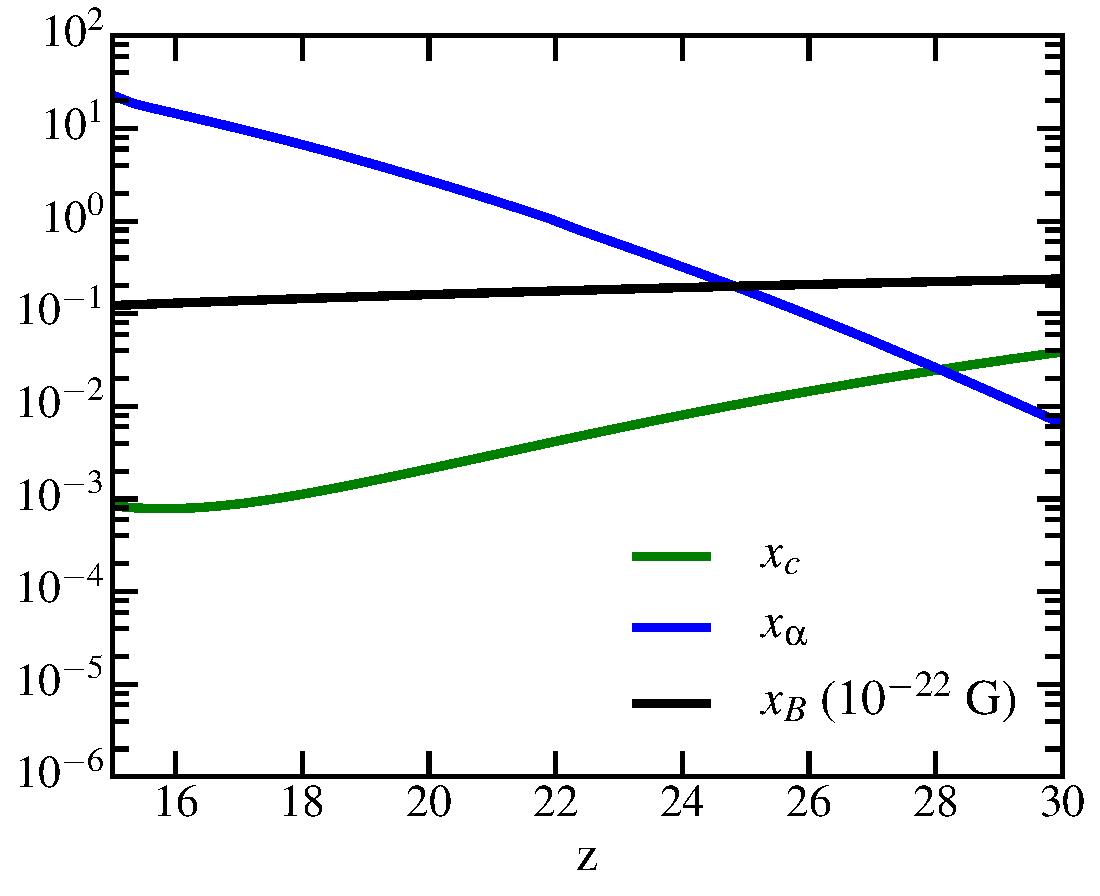
\includegraphics[width=.35\textwidth,keepaspectratio=true]{xs.pdf}
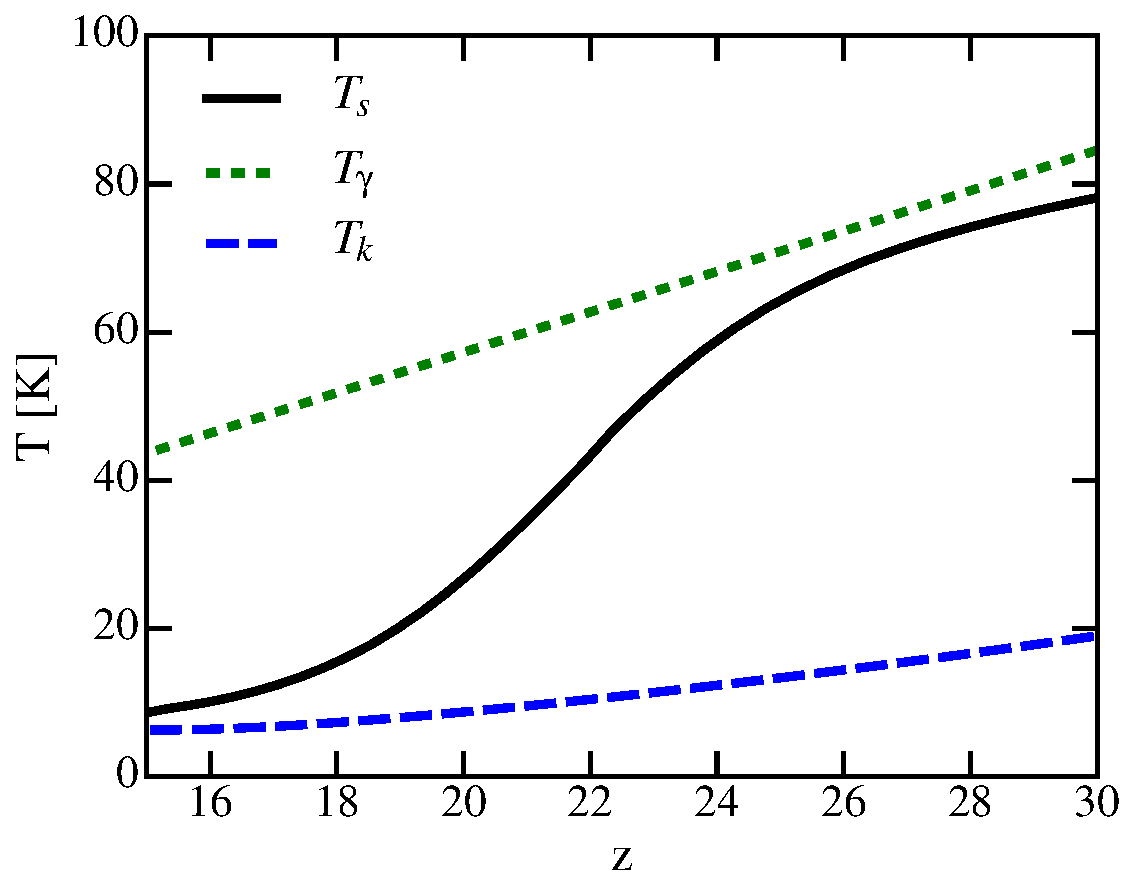
\includegraphics[width=.35\textwidth,keepaspectratio=true]{Ts.pdf}
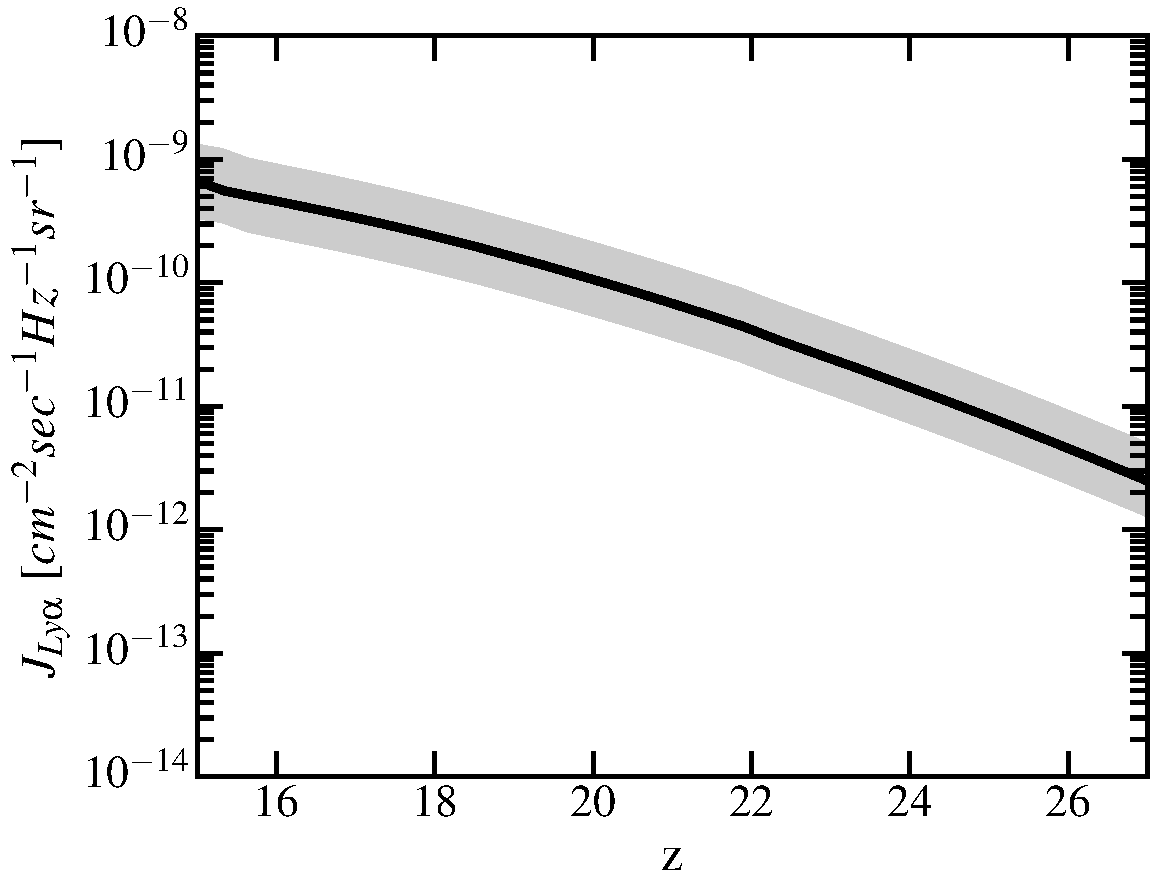
\includegraphics[width=.35\textwidth,keepaspectratio=true]{Jlya.pdf}
\caption{Inputs used for the sensitivity calculation, computed for standard cosmology using \texttt{21CMFAST} code. Top panel: fiducial spin, kinetic, and CMB temperatures. Middle panel: fiducial models for quantities that parametrize the rate of depolarization of the ground state by optical pumping and atomic collisions, and the rate of magnetic precession for a representative value of the magnetic field. Bottom panel: Lyman-$\alpha$ flux model; fiducial choice is shown with a solid line, while the gray band captures the level of modeling uncertainty (it spans of the ``extremal'' input models used to test sensitivity of our calculation to this uncertainty, as discussed in the text). \label{fig:cosmo}}
\end{figure}
We now proceed to numerically evaluate the sensitivity of 21--cm tomography to magnetic fields during the pre--reionization epoch, using the formalism from previous two Sections. For this purpose, we only focus on one type of experimental setup---an array of dipole antennas arranged in a compact grid, such as implemented in HERA, for example. The motivation for this choice is that such a configuration maximizes sensitivity to recovering the power spectrum of the cosmological 21--cm signal \cite{2009PhRvD..79h3530T,2015AAS...22532803D}. We consider an array with a collecting area of $(\Delta L\text{ km})^2$, where $\Delta L$ is taken to be the maximal baseline separation.

Calculationg of the observation time $t_1$ (appearing in the expression for the noise in Eq.~(\ref{eq:Pnoise_K})), for a given total survey duration $t_\text{obs}$, depends on the type of the experiment.  For a radio dish with a beam of solid angle $\Omega_\text{beam}=\lambda^2/A_e$ that is much smaller than the survey size $\Omega_\text{survey}$, the telescope scans the sky one beamwidth at a time. In that case, $t_1$ is the total time spent observing one $(u,v)$ element $t_1=t_\text{obs}\Omega_\text{survey}/\Omega_\text{beam}$. However, in the case of an array of dipoles we are considering here, the beam size is greater than (or equal to) the survey size, and $t_1=t_\text{obs}$. We do not explicitly account for the fact that any given patch of the sky is only visible for a part of the day from a given location; therefore, $t_\text{obs}$ we substitute in the noise calculation is shorter than the wall--clock duration of the survey by a factor of a few. To derive numerical results, we assume $\Omega_\text{survey}=1$sr, and the wall--clock survey duration of about 2 years (corresponding to $t_\text{obs}=1$ year). 

For the sky temperature that enters the noise power spectrum in \eq{\ref{eq:Pnoise_K}}, we assume a simple model of Galactic synchrotron emission from Ref.~\cite{2008PhRvD..78b3529M}, 
\beq
T_\text{sky}  = 60\left(\frac{21}{100} (1+z)\right)^{2.55}\text{   [K]}.
\label{eq:tsys}
\eeq

Other ingredients entering our sensitivity calculation are the mean Lyman--$\alpha$ flux $J_{\text{Ly}\alpha}(z)$, the spin $T_s$ and the kinetic $T_k$ temperatures of the IGM, and the CMB temperature $T_\gamma$, all functions of redshift. We obtain all of these quantities from \texttt{21CMFAST} code \cite{2011MNRAS.411..955M}. As input to \texttt{21CMFAST}, we used standard cosmology ($H_0=67$ km s$^{-1}$ Mpc$^{-1}$, $\Omega_\text{m}=0.32$, $\Omega_K=0$, $n_s=0.96$, $\sigma_8=0.83$, $w=-1$) consistent with Planck measurements \cite{2015arXiv150201589P}, set the stellar population responsible for early heating to Population III, and kept all other input parameters at their default values, with the exception of the star formation efficiency, \verb|F_STAR|. For our fiducial calculation, we choose the value of \verb|F_STAR|=$0.0075$, corresponding to the solid lines in Figure \ref{fig:cosmo}. The top panel shows quantities (discussed in Paper I) that parametrize the rates of depolarization of the ground state by optical pumping and atomic collisions, and the rate of magnetic precession. The middle panel shows the relevant gas and CMB temperatures. The bottom panel shows $J_{\text{Ly}\alpha}(z)$, where the solid line, as before, corresponds to the fiducial choice of parameters, while the gray band of ``uncertainty'' around this curve corresponds to \verb|F_STAR|$=0.0025$ and \verb|F_STAR|$=0.01875$. The fiducial choice produces a match of the flux to the models in Ref.~\cite{2012ApJ...746..125H} at $z=15$, while the gray band is chosen to roughly capture the level of the uncertainty in the flux modeling at high redshifts (given the lack of direct observation at high $z$). We use these extreme models (corresponding to the bounds of the gray band in this Figure) to test sensitivity of our key results to the uncertainty in the evolution of the Lyman--$\alpha$ flux and other input parameters (note that we do not plot corresponding uncertainty bands on the other two panels, simply to avoid clutter; but we use them consistently in our sensitivity calculation). We assume that the redshifts available for this analysis are between $15$ and $35$. As we will see from Figure \ref{fig:Bsat} (discussed in more detail below), most of the sensitivity comes from redshifts where the spin temperature starts decoupling from the CMB; for our fiducial case, it is around $z\sim 21$. 

\begin{figure}
\centering
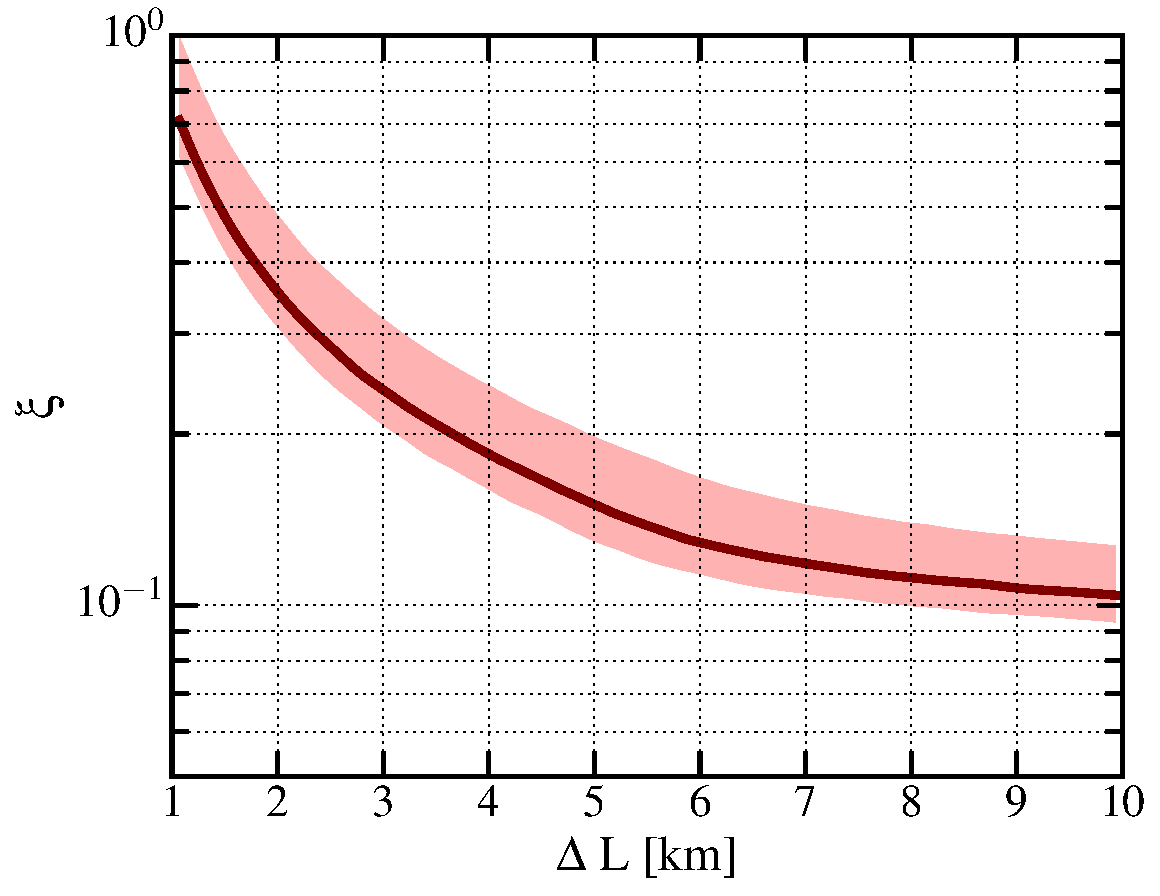
\includegraphics[width=.35\textwidth,keepaspectratio=true]{xi_vs_deltas.pdf}
\caption{Projected sensitivity to detecting a magnetic field in the saturated regime, as a function of the maximum baseline (or, equivalently, of the total collecting area, ($\Delta L)^2$), assuming a survey size of 1 sr and survey duration of 2 years. The parameter on the $y$ axis characterizes the distinction between the case of no magnetic field ($\xi=0$) and the presence of a strong field ($\xi=1$). Smaller values here (for larger maximum--baseline values shown on the $x$ axis) correspond to more precise recovery of $\xi$ and a more confident distinction between those two regimes. The light--colored band around the solid line corresponds to the Lyman-$\alpha$ model flux uncertainty, represented with a gray band in Figure \ref{fig:cosmo}.\label{fig:xi_vs_deltas}}
\end{figure}
\begin{figure}
\centering
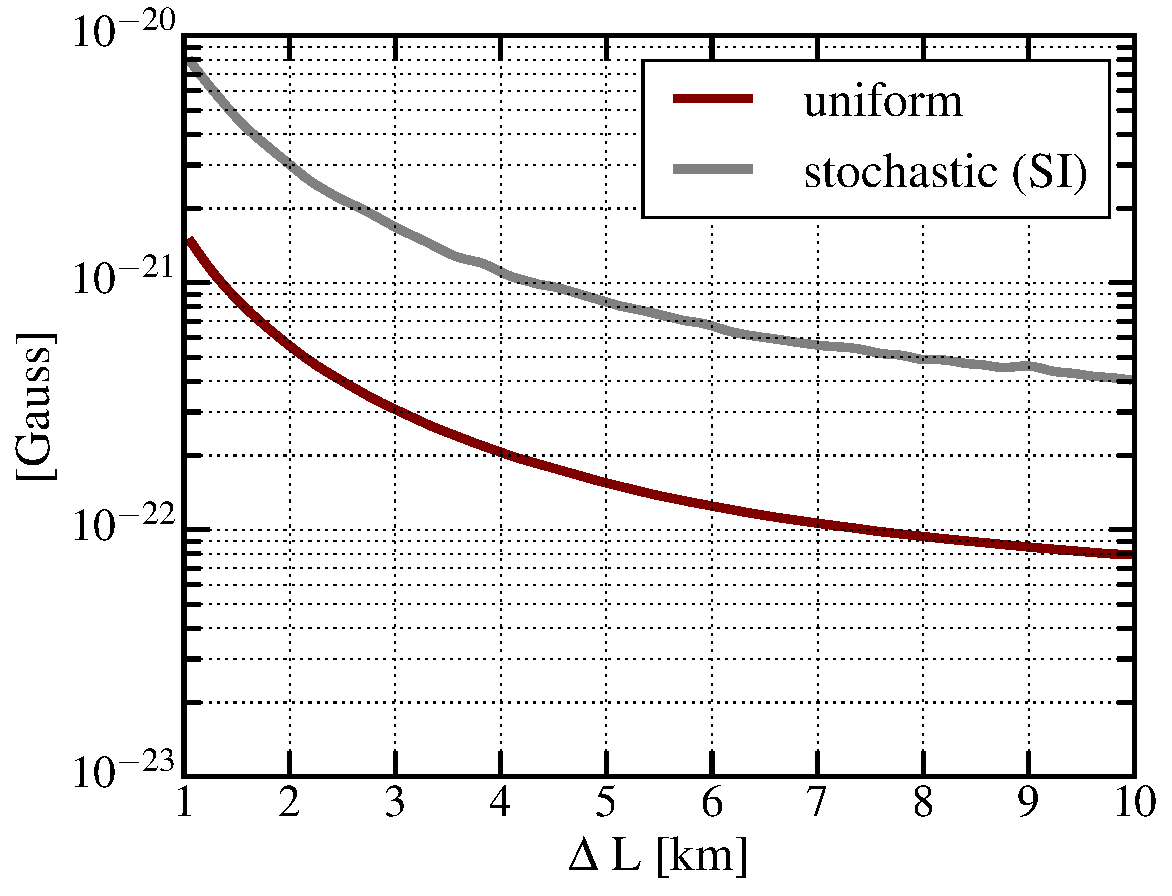
\includegraphics[width=.35\textwidth,keepaspectratio=true]{B_vs_deltas.pdf}
\caption{Projected $1\sigma$ sensitivity to detecting a uniform (lower red line) and a stochastic (upper gray line) magnetic field, as a function of maximum baseline $\Delta L$ (the collecting area of the array is given as $(\Delta L)^2$).  For the stochastic field, we assume a scale--invariant (SI) power spectrum, and show the root--mean--squared variation per $\log K$, given by $A_0/\pi$, where $A_0^2$ is the amplitude of the power in a transverse component), as a function of maximum array baseline, assuming a survey size of 1 sr, and for survey duration of 2 years.\label{fig:B_vs_deltas}}
\end{figure}
Figures \ref{fig:xi_vs_deltas} and \ref{fig:B_vs_deltas} show the key results: the projected sensitivity of tomographic surveys as a function of the maximum baseline $\Delta L$ (where different baselines may correspond to different stages of a single experiment). Figure \ref{fig:xi_vs_deltas} shows $1\sigma$ sensitivity to parameter $\xi$ of \eq{\ref{eq:saturated_P}}, which quantifies the distinction between the case of no magnetic field and the case where the field is strong and the signal is in the saturated regime. The value of this parameter is, by definition, bound between 0 and 1, where 0 represents the case of no magnetic field, and 1 represents the saturated case. In this Figure, the solid line represents the fiducial calculation, while the light--colored band around it corresponds to the uncertainty band of inputs shown in Figure \ref{fig:cosmo}. The fiducial result implies that an array with one kilometer squared of collecting area can achieve $1\sigma$ detection threshold, which can be interpreted as follows. If a survey were to measure $\xi\ne 0$, that would be a $1\sigma$ detection of a lower bound on a uniform magnetic field in the entire survey volume. The value of the lower bound as a function of redshift would correspond to the saturation ceiling at that redshift, which can be roughly evaluated from the condition that the depolarization rates through standard channels equal the rate of magnetic precession, $x_B = 1+x_{\alpha ,(2)} +x_{c,(2)}$. The ceiling is depicted with a dashed line in Figure \ref{fig:Bsat}, and it corresponds to $|\vec B|\sim 2\times 10^{-21}$ Gauss (comoving) at $z=20$, for example.  On the other hand, if a survey were to report a null result, it would rule out such a magnetic field, at the same confidence level. In that case, we can compute an upper bound on the strength of the magnetic field components in the plane of the sky, as discussed in the following. 

We obtain results in Figure \ref{fig:B_vs_deltas} by evaluating the expressions of Eqs.~(\ref{eq:fisher_patch}) and (\ref{eq:snr_ints}). This Figure shows a projected $1\sigma$ upper bound that can be placed on the value of the magnetic field, in case of no detection with an array of given size. The result is shown for both the uniform field (lower solid red line), and for the amplitude of a stochastic field (upper gray line) with a scale--independent power spectrum. While the numerical calculation assumed that the brightness temperature is a linear function of the field strength, this assumption is not guaranteed to hold---it breaks down in the saturation limit, as discussed above and in \S\ref{sec:method}. So, this Figure is only valid if $\xi=0$.

In order to understand how the projected constraints (sensitivities) presented in Figure \ref{fig:B_vs_deltas} compare to the saturation ceiling at the redshifts we consider, Figure \ref{fig:Bsat} shows a comparison between the saturation ceiling and the values of the $z$--dependent integrands of \eq{\ref{eq:fisher_patch}} (plotted for several array sizes). We can now see that the sensitivity to the uniform field corresponding to all array sizes in consideration is below the saturation regime for the redshifts where most of the SNR comes from: $z\sim21$ (the minima of these curves). This gives us confidence that the results for the uniform field in Figure \ref{fig:B_vs_deltas} are indeed valid, and the linear theory holds in the given regime (the transfer function is a linear function of the field strength). For the stochastic case, however, it is likely that a factor of a few larger array sizes are needed to achieve sensitivity that is below the saturation limit at relevant redshifts. It is also important to note here that the calculation of the saturation ceiling presented in this Figure is quite conservative, where in reality linear approximation should hold well until the field reaches a value that is a few times above this level.
\begin{figure}
\centering
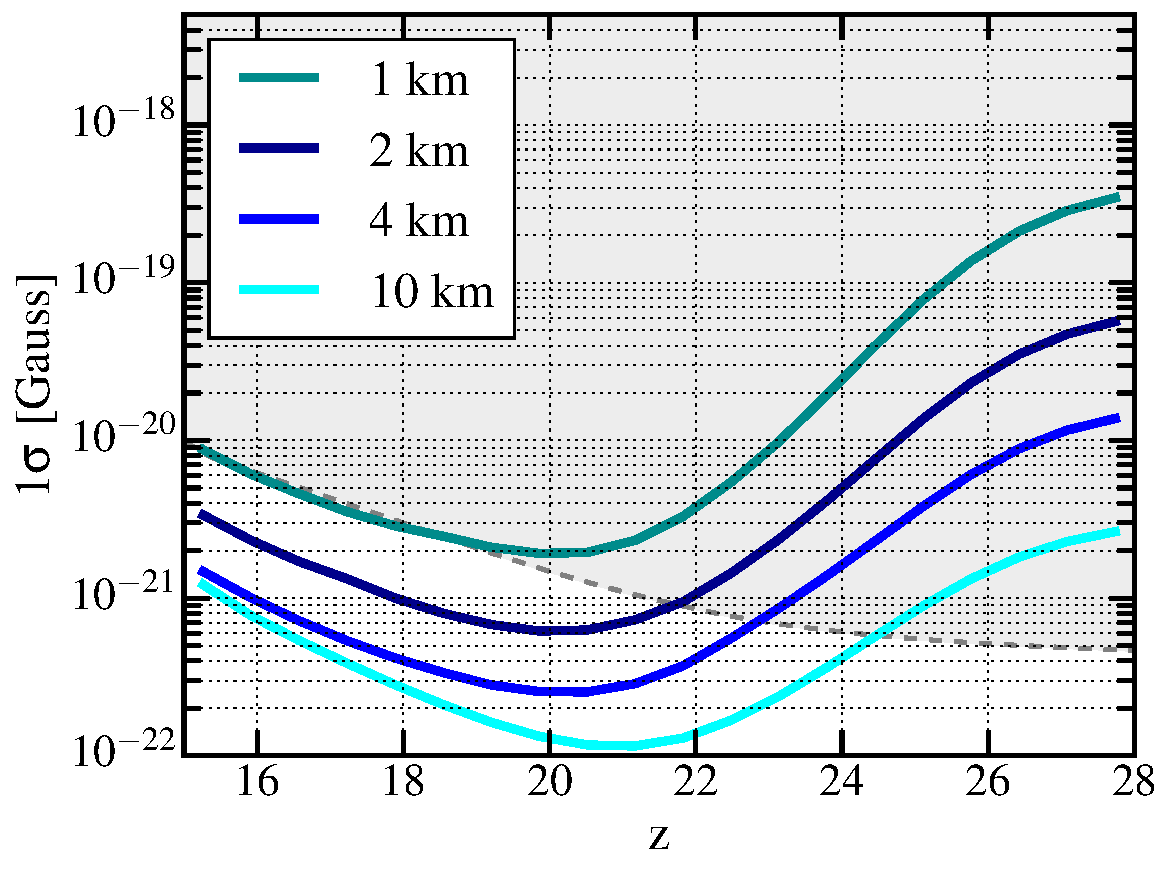
\includegraphics[width=.35\textwidth,keepaspectratio=true]{sigmaB0_vs_z.pdf}
\caption{Saturation regime is shown as a shaded gray area above the dashed curve. Integrand of \eq{\ref{eq:fisher_patch}} (inverse sqare root of it) is shown as a function of redshift, for several maximum---baseline lengths.  When the colored curves are below the saturation limit around their minima, the analysis assuming unsaturated regime is valid.\label{fig:Bsat}}
\end{figure}
